
\documentclass[runningheads]{llncs}
%
\usepackage{graphicx}
\usepackage{gensymb}
\usepackage{mathtools}
\usepackage{float}
\usepackage{listings}
\usepackage{blindtext}
\begin{document}
%
\title{Smart Energy Systems Lab: Electricity Demand-Response Managements}

\author{Muralikrishna Thulasi Raman \and
Tung Dinh \and
Shaiori Saha}

\institute{Service Computing Department, IAAS, University of Stuttgart}
%
\maketitle              % typeset the header of the contribution
%
\begin{abstract}
This report gives a detailed information on the lab results of ``Smart Energy Systems Lab: Electricity Demand-Response Management''. This gives us information on existing functionality of the microgrid, challenges involved, features that can be added on the existing architecture. Microgrid works as a local energy provider for domestic buildings to reduce energy expenses and gas emissions by utilizing distributed energy resources (DERs). The rAPId advances in computing and communication capabilities enable the concept smart buildings become possible. Most energy-consuming household tasks do not need to be performed at specific times but rather within a preferred time. If these types of tasks can be coordinated among multiple homes so that they do not all occur at the same time yet still satisfy customers’ requirement, the energy cost and power peak demand could be reduced.  
\keywords{Micro grid  \and Smart grid \and Dynamic pricing \and gurobi.}
\end{abstract}

\section{Introduction}
Due to the increase of energy demand and rising global emissions of greenhouse gases the future electricity distribution system should be designed in such a way that it is  integrated, intelligent and better known as smart grid, which includes advanced digital meters, distribution automation, communication systems and distributed energy resources.\cite{Efficiency} 
\newline
Micro grids are small scaled localized energy network which include load ,network control system, generators and energy storage devices. Micro grids face major technical challenges  with respect to voltage and frequency control, islanding  and protection of micro grids.\cite{Microgrid}
\newline
In electricity system, the unbalanced condition between  active and reactive power generated and power consumed by the loads including the losses in the lines  occurs due to the difference between the power generated and the power demanded.Once a micro grid is formed  it is important to assure the loads, lines and the distributed generation on the island are protected.\cite{Efficiency}
\newline
We want to design our smart energy system that provides a web based interface to the user for real time simulation that includes modelling Supply and Demand side, Dynamic Pricing, Demand Response and Coordination, visualization with a view to optimizing asset utilization, minimizing operations and maintenance cost and low-carbon/low-pollutant generation.\cite{Efficiency}

\section{Overview}
The architecture of the entire system is given in the figure  given below.
\begin{figure}[H]
\centering
\includegraphics[width=0.7\textwidth]{{"actual/architecture"}.png}
\caption{The architecture of the system with all the components involved} 
\label{fig2}
\end{figure}

From the upper figure, the function and interaction of modules can be deduced: 
\begin{itemize}
    \item Weather Service: uses data from Weatherbit.io API to provide the current and forecast of 24 hours weather data. This service has the capability to get latest data for the current hour through last update time check (both for current data and forecast data)
    \item Supply Service: when requested (either from optimisation service or UI), this web service uses data from Weather Service and calculates energy generated from Simulated Wind Turbine and PV components, stores them in the Database and gives data to the requested module. Apart from these, it updates, stores and retrieves battery data. Not to forget, new Wind turbine and solar panel can be added to the system through this service. Also, battery specifications can be updated.
    \item Demand Service: when requested, Demand Service which is an web service gets information like building's energy consumption [both total and controlled devices energy consumption]. Also, new buildings and devices can be added into the system through this service. Also, it has the capability to update device information like Start Time, Stop Time which is used by optimisation service to operate the devices towards the optimisation goal. 
    \item Pricing Unit: is also a web service that provides us with pricing data of energy 
    \begin{itemize}
        \item For current hour
        \item For current day's 24 hours
        \item For next day's 24 hours
        \item Forecast for the next 24 hours
    \end{itemize}
    \item Optimisation: uses data from Supply Service, Demand Service and Pricing Unit to optimise the system towards the goals. It uses Gurobi module to optimise the operation of devices in building. Once optimum schedule is obtained, the start and end time of devices are updated in the Demand Side through the web service interface. Also, battery data is updated through supply side Service.
    \item User Interface UI: is created using NUXT JS (a framework based on Vue JS) and Vuetify (Material design CSS Framework for VUE JS) \cite{Vuejs}. This unit has fluidic design, interactive charts and forms to obtain information from user and also to display information from Supply Service, Demand Service, Pricing Unit and Optimisation unit.
\end{itemize}

\section{Supply Side}
In this section we show the implementation of several components of our system that will simulate the supply side of the microgrid. We  have chosen Weatherbit.io that provides current weather data and forecast of  24 hours of weather data for a given location(in our case Stuttgart) on an hourly basis.It provides the highest quality weather forecasts, observations.uses global forecast models (GFS/ECMWF), in combination with local short range high resolution models such as the HRRR, the NAM, and the DWD ICON models to derive the most accurate forecast data possible. Data retrieved from weather API\cite{Weatherbit.io} service contains the following:

\begin{itemize}
\item Temperature in $\degree$Celsius 
\item Wind speed in m/s
\item Pressure of (dry) air in  Pascal
\item Relative humidity in \%
\item Solar irradiance in $W/m^2$
\item Latitude in $\degree$
\item Day of year
\end{itemize}

For power generation we are dependent on Solar panel and Wind turbine.\\
\subsection{Wind Turbine}
Wind turbine converts the kinetic energy from the Wind into rotational kinetic energy which is then converted to electrical energy by an electricity generator. The power in the Wind that can be extracted by a Wind turbine is proportional to the cube of the Wind speed :\cite{Ilche}\\
\[P(t)= \frac{1}{2} \times \rho A \mathnormal{U(t)^3}C_p \;\;[W]\] 
\newline
where:
\begin{itemize}
\item $\rho$ is air density in $kg/{m^3}$
\item $A=\; \pi \times Ra^2$ is the rotor swept area in $\mathnormal{m^2}$
\item Ra is radius of blade in m
\item U(t) is Wind speed in m/s
\item $C_{p}$ is a power coefficient that represents the aerodynamic efficiency of the rotor in percentage. Theoretically it has a maximum value of 0.59, but due to engineering constraints, practically its value lies from 0.35 to 0.45. In our case we have taken  an average of 0.35 and 0.45 which equals to 0.4.\\
\end{itemize}

{\raggedleft To calculate air density we take following into consideration:}\\
\[\rho=\mathrm{\rho}_d{}_a{}+\mathrm{\rho}_v{}\]
\newline
where:
\begin{itemize}
\item $\rho_{da}$ is the partial density of dry air.
\item $\rho_{v}$ is the partial density of water vapor.\\
\end{itemize}
The partial density of dry air in humid air is:\\
\[\mathrm{\rho}_{da}= \frac{p_{da} \times M_{da}}{RT}\]\\
where:
\begin{itemize}
\item $p_{da}$ is the partial pressure of the dry air.
\item $M_{da}$ is the molar mass of the dry air (0.0290kg/mol).
\item R is the ideal gas constant(8.314 J/molK).
\item T is the temperature in degrees Kelvin.
\end{itemize}
The partial density of water vapor in humid air is:\\
\[\mathrm{\rho}_{v}= \frac{p_{v} \times M_{v}}{RT}\]\\
where:
\begin{itemize}
\item $p_v$ is the partial pressure of the water vapor.
\item $M_v$ is the molar mass of the water vapor (0.0180kg/mol).
\item R is the ideal gas constant (8.314 J/molK).
\item T is the temperature in degrees Kelvin.
\end{itemize}
In order to find out partial pressure of water vapor we have:\\
\[Relative Humidity(RH)=\frac{p_{v}}{p_{v}'(T)}\]\\
where
\begin{itemize}
\item $p_{v}$ is the partial pressure of water vapor.
\item $p_{v}'$(T) is the saturated vapor pressure at a temperature of T.
\end{itemize}
Using Teten's formular, $p_{v}'$ is calculated: $p_{v}' = c_{0} \times 10^\frac{c_{1}\times T}{c_{2}\times T} $, in which: 
\begin{itemize}
    \item T $\degree$Celcius
    \item $c_{0} = 6.1087$
    \item $c_{1} = 7.5$
    \item $c_{2} = 273.3$
\end{itemize}

From the API we get current value and forecast of 24 hours for temperature, pressure, humidity and Wind speed and user inputs the radius of the rotor. Then using the above formula mentioned we calculate current  Wind power and forecast of generated power for next 24 hours. One small notice for coding part, the pressure collected from API is assumed to be dried air pressure $p_{da}$. \\
%$a\textprime$
\subsection{Photo Voltaic}
Photo Voltaic converts sun light into electricity using solar cells.From the Web API we get current value and forecast of 24 hours for temperature,latitude,day of year and solar irradiance and user inputs the angle of module and area of solar panel.Then using the above formula mentioned we calculate current solar power and forecast of generated power for next 24 hours.Power generated by a photovoltaic is calculated  using the following formula:\\
\[P(t)=A \times \eta \times PR(t) \times S(t) \;\;[W]\]\\ 
where
\begin{itemize}
\item A is the surface area of the solar cells in $\mathnormal{m^2}$.
\item $\eta = E_{max}$/A (in \%)  is the power efficiency coefficient of the solar panel in percentage(Watt-peak).
\item PR(t) is is a performance ratio in percentage.
\item $S(t) = \frac{S_{horizontal} \times \sin(\alpha +\beta)}{sin(\alpha)} $ is the solar irradiance in $W/\mathnormal{m^2}$. Solar irradiance is the power received from the sun and depends on the angle
between the panel and the sun \cite{Irradiance}, where:
\begin{itemize}
\item Angle of module ($\beta$) is user input.
\item Angle of Sun ($\alpha$)=90-$\phi$+$\delta$.
\item $\phi$ is latitude obtained from Weather API.
\item $\delta = 23.45\times\sin(360(284+day\_of\_year)/365)$
\end{itemize}
\end{itemize}
Accounting  for a variety of losses, such as cable losses, losses at weak radiation,temperature losses, losses due to  cloud coverage, etc we consider \\
%\centerline{sentence should be centered.}
\centerline{PR=$L_T$+$L_0$}\\
Where $L_T$ is the temperature loss (in $\degree$Celcius) and $L_0$ is a constant loss of 14\% accounting for other types of losses.\\


\subsection{Battery}
Battery is used to store the excess charge from generation unit i.e  if we have excess amount of energy from PV or Wind Turbine after fulfilling the demand,we can store it  for further usage.Battery has two action:charge and discharge but this cannot be done simultaneously.Battery unit has three states-Charge ,Discharge and Idle.While charging, output power is indicated negative and while discharging it is shown with positive value.The energy of a battery at time t:\\
\[E(t)=E(t-1)+ (\delta.\eta.E_{CH}(t))-(\delta.E_{DCH}(t)/\eta)-(\delta.s(t).E_{SELF})\]
where
\begin{itemize}
\item $\delta$ is time interval duration.
\item $\eta$ is the battery efficiency.
\item $E_{CH}$(t) is charge at time t.
\item$E_{DCH}$(t) is discharge at time t.
\item s(t) is the battery status at time t.It is 1 if battery is ON and 0 when battery is OFF.
\item $E_{SELF}$ is the self-discharging rate of the battery.
\end{itemize}
To prevent net accumulation, the battery must return to its initial value at the end of each day.\\
In order to maintain the storage and avoid damaging/reducing capacity\\
%a\textsuperscript{th}\\ $\leq$ 
\begin{itemize}
\item $E_{CH}$(t)$\leq$ $E_{CH}$\textsuperscript{SPECS}
\item $E_{DCH}$(t)$\leq$ $E_{DCH}$\textsuperscript{SPECS}
\item E(t)$\leq$ E\textsuperscript{SPECS}
\end{itemize}
where
\begin{itemize}
\item $E_{CH}$\textsuperscript{SPECS}is the upper bound of battery charge rate.
\item $E_{DCH}$\textsuperscript{SPECS}is the upper bound of battery discharge rate.
\item E\textsuperscript{SPECS}is the upper bound of battery energy.
\end{itemize}
\textbf{Implementation:}
\centerline {Now we show how we have implemented Supply side module in our system:}
\begin{figure}[H]
\centering
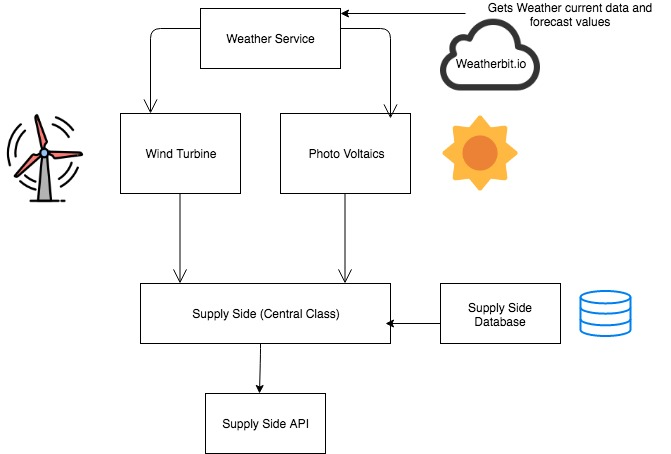
\includegraphics[width=0.4\textwidth]{actual/supplyside.jpg}
\caption{Implementation of Supply Side} 
\label{fig3}
\end{figure}
\medskip{}
{\raggedleft \textbf{SupplySide Central Class:}}
\begin{itemize}
    \item Default method to add supply side with  default modules.
    \item We can add a module for Wind turbine model.
    \item We can add a module for solar energy.
    \item We have the provision to get the battery data and update battery data(e.g  state,charge) in database.
    \item We get current energy generation data for Wind,PV and total energy generation.
    \item We get forecast energy generation data for Wind,PV and total energy generation.
    \item When methods are called there is  a last update check that tells whether data is latest for that hour.If so, it returns the data.
\end{itemize}

{\raggedleft \textbf{SupplySide API:}}
Here we have used Bottle  web framework which is licensed under MIT license.From bottle we have imported  route,run, request.\cite{bottlepy}The route() decorator binds a piece of code to an URL path.During development, we have to restart the server a lot to test recent changes.This can be done using auto reloader.Every time a module file is edited, with help of run() decorator the reloader restarts the server process and loads the newest version of the code.With request() decorator we can perform  GET, PUT, POST actions.
\begin{table}[H]
\centering
\caption{Routes of Supplyside API}\label{tab1}
\begin{tabular}{|p{3.5 cm}|p{8.5 cm}|}
\hline
\textbf{Routes} & \textbf{Roles} \\
\hline
'/supplySideInitialise' & If there is input ,the modules(Wind,PV,Battery) are initialized. Otherwise, default module from predefined specifications will be initialised\\
\hline
'/Windcurrentenergy' & Shows the  current generated power by Wind module.\\
\hline
'/PVcurrentenergy' & Shows the  current generated power by PV module.\\
\hline
'/addWind' & User can add a new Wind module.\\
\hline
'/addPV' & User can add a new Wind module.\\
\hline
'/addBattery'  & User can add a Battery.\\
\hline
'/getWindEnergyData' & User gets the  current and forecast  values of Wind power.\\
\hline
'/getSolarEnergyData' & User gets the  current and forecast  values of solar power.\\
\hline
'/totalcurrentenergy'  & User gets the sum of power generated at current  hour from PV and Wind  module.\\
\hline
'/getBatteryData' & User can get the data for battery module.\\
\hline
'/Windforecastenergy'  & User  gets the forecast of 24 hours of power generated by Wind.\\
\hline
'/PVforecastenergy' & User gets the forecast of 24 hours of power generated by PV.\\
\hline
'/totalforecastenergy' & User gets  the sum of forecast of 24 hours of power generated by PV and Wind.\\
\hline'/updateBatteryData' & It  is used to update battery state and  charge\\
\hline
\end{tabular}
\end{table}

\begin{table}[H]
\centering
\caption{Tables of Supply Side schema}\label{tab2}
\begin{tabular}{|p{3 cm}|p{8.5 cm}|}
\hline
\textbf{Tables} & \textbf{Columns} \\
\hline
WindModules & Id, Status, SupplySide, Location, Current Energy, Forecast Energy, Ra(Radius of rotor blade).\\
\hline
SupplySide &Id, Description.\\
\hline
PVModules & Id, Status, SupplySide, Area, Emax, Angle of Module, Location, Current Energy, Forecast Energy.\\
\hline
LastUpdate & Id, LastUpdate.\\
\hline
Battery & Id, Status, SupplySide, State, Efficiency, TimeInterval, InitialEnergy, SelfDischargeRate, Charge, ChargeSpecs, DischargeSpecs, EnergySpecs.\\
\hline
History & Hour, WindEnergy, SolarEnergy, TotalEnergy.\\
\hline
\end{tabular}
\end{table}

\section{Demand Side}
In demand side we have implemented a component Building which consists of  uncontrollable devices and controllable devices.For uncontrollable devices we have used demand profile based on historical data provided by \texttt{https://open-power-system-data.org/}.
The controllable devices(Controllable Electrical Devices) can be scheduled using an  optimized schedule (which has been implemented  in Optimization unit) based on economical and technical constraints.User can specify the starting time, end time and length of operation.Total demand of a building comprises of the sum of Controllable devices demand and uncontrollable devices demand.\\ 
\subsection{Controllable Devices(CED)}
To model the controllable devices we have used following parameters and constraints.\\
\textbf{Parameters:}\\ 
\begin{itemize}
\item Earliest start time(EST)  in hour.
\item Latest End time(LET) in hour.
\item Length of operation time (LOT)in hour.
\item Power(E) in  kilowatt(kW).
\end{itemize}
\textbf{Constraints:}\\
\begin{itemize}
    \item Operation time of each device must be within the provided time Window, and
each device must be started once and subsequently finished once.
\item Device should  be in OFF status before EST  and after LET.It should only be ON once during EST and LET.
\item In order to operate, device should be turned on.
\item Device should operate for LOT hours before it is turned off.
\item Device should operate exactly same amount of time as LOT.
\end{itemize}
\subsection{Uncontrollable Devices}
They are modelled via an aggregated load profile based on historical data obtained from \texttt{https://open-power-system-data.org/}.We have chosen the household data package  that contains  measured time series data for several small businesses and private households relevant for household- or low-voltage-level power system modeling.The data includes electricity consumption (load) in a resolution up to single device consumption on hourly basis.\cite{Opsd}
\subsection{Building}
Building comprises of controllable and uncontrollable devices.Thus the total power consumption demand for a specific building is  sum of power consumption of controllable devices of the building  and power consumption of  uncontrollable devices of the building.Thus  the total electrical demand of a building at time t is:\\
%\textsuperscript{SPECS}
\centerline{D(t)=D\textsuperscript{UD}(t)+D\textsuperscript{CED}(t)}\\
where D\textsuperscript{UD}(t)is the electrical power demand of uncontrollable devices at time t.\\
D\textsuperscript{CED}(t)is the electrical power demand of controllable electrical devices at time t.\\
\textbf{Implementation:}\\
\centerline {Now we show how we have implemented demand side module in our system:}\\
\begin{figure}[H]
\centering
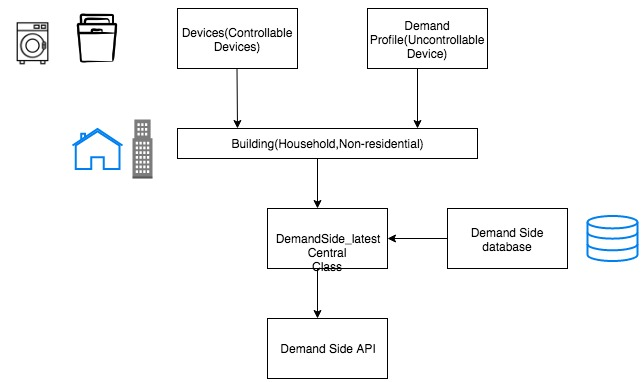
\includegraphics[width=0.7\textwidth]{actual/demandside.jpg}
\caption{Implementation of Demand Side} 
\label{fig3}
\end{figure}

{\raggedleft \textbf{DemandSide Central Class:}}
\begin{itemize}
    \item User can add a demand side module.
    \item User can add building.
    \item User can add  one or multiple device to a building.
    \item User can get building list  based on demand side id.
    \item User can get building details based on building id.
    \item User can  get device details(EST,LOT,LET,power consumption,start time,end time,device status etc.) based on building id.
    \item User can get device details based on device id.
    \item User can update building data based on modified  power consumption of devices.
    \item User can update device data based on modified  power consumption.
    \item User can update start and stop time of the  controllable device.
\end{itemize}
{\raggedleft \textbf{DemandSide API:}}\\
\begin{table}[H]
\centering
\caption{Routes of Demandside API}\label{tab1}
\begin{tabular}{|p{5 cm}|p{8.5 cm}|}
\hline
\textbf{Routes} & \textbf{Roles} \\
\hline
'/demandSideInitialise' & If there is input, the modules(buildiing, devices) are initialized. Otherwise, default module from predefined specifications will be initialised.\\
\hline
'/addDevice' & User can see device with EST, LET, power, LOT, name, StartTime, EndTime, BuildingId.\\
\hline
'/addBuilding' & User can add building.\\
\hline
'/buildings' & User can see list of buildings added to a demand side.\\
\hline
'/getAllDevices' & User can get all devices list.\\
\hline
'/devices' & User can get all devices  for a particular building.\\
\hline
'/building' & User can get the building details based on building id.\\
\hline
'/updateStartStopTimeDevice' & User can update start time  and stop time  of a device.\\
\hline
\end{tabular}
\end{table}
{\raggedleft \textbf{DemandSide Database:}}
\begin{table}[H]
\centering
\caption{Tables of Demand Side schema}\label{tab2}
\begin{tabular}{|p{2.5cm}|p{9cm}|}
\hline
\textbf{Tables} & \textbf{Columns} \\
\hline 
DemandSide  & Id,Description.\\
\hline
LastUpdate & Id,LastUpdate.\\
\hline 
Building & Id, DemandSide, BuildingName, CED\_Count, CED\_List, CEDConsumption, UDConsumption, TotalDemand.\\
\hline 
DeviceModules  & Id,Building, DemandSide, DeviceName, EST(h), LET(h), LOT(h),Power(kW), StartTime(h), EndTime(h), DeviceStatus, Power\_total(Kw), Power\_sum(Kw).\\
\hline
\end{tabular}
\end{table}
\section{Dynamic Pricing}
This project depicts USA market model, in which, the electric price fluctuates the whole day every single hour. Assignment 3 requires to store 24 pricing values of day-ahead-market, in case they are at the time not available, the previous ones are taken into account.

In response to the request, the pricing service including pricing and pricing\_app work as backbone and API of the service. Not only day-ahead pricing data, but also current day and forecast data, which are 24 values from the hour user pull pricing extract request. Pricing database can be well observed in pricing\_data ,in which, there are 3 tables about latest update time, 24-value current day and day-ahead tables.

\begin{figure}[H]
	\centering
	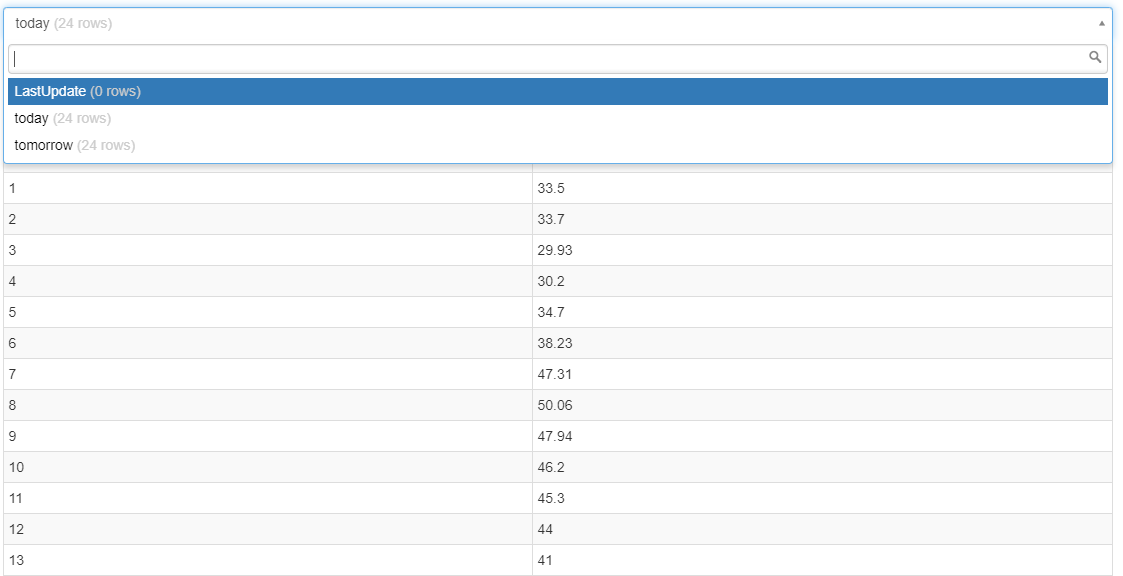
\includegraphics[width=0.7\columnwidth]{pricingdb.png}
	\caption{The pricing database}
	\label{img:control_database}
\end{figure}

Because of the stability and reliability in bidding region and pricing data, this project use Belgium pricing data, which is slightly different in detail comparison. German data, on the other hand, has some unexpected problems during trial on different computers, it is somehow got "key error" problem. To use data from Germany, key word has to be changed to "DE-LU" for data later than 10/2018, since the bidding zone changed from "DE-LU-AT" to "DE-LU" which is sometimes conflict, and time function has to be changed to utc. Below is 2 code test for normal and special German usages. \newline

\begin{figure}[H]
	\centering
	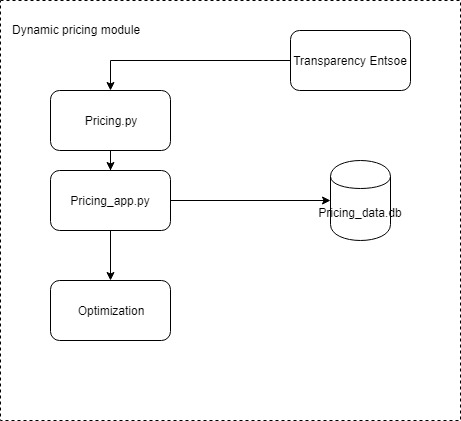
\includegraphics[width=0.7\columnwidth]{pricing.jpg}
	\caption{The pricing module}
	\label{img:control_module}
\end{figure}

\begin{lstlisting}
from entsoe import EntsoePandasClient
import pandas as pd
from datetime import datetime

client = EntsoePandasClient(API_key=<YOUR API KEY>)

start = datetime.now().date().strftime('%Y%m%d')
end = (datetime.now().date()+ timedelta(days=1)).strftime('%Y%m%d')
country_code = 'BE'  # Belgium

# methods that return Pandas Series
client.query_day_ahead_prices(country_code, start=start,end=end)
\end{lstlisting} 

\medskip
{\raggedleft and for Germany-Luxembourg}
\medskip

\begin{lstlisting}
from entsoe import EntsoePandasClient
import pandas as pd
from datetime import datetime

client = EntsoePandasClient(API_key=<YOUR API KEY>)

start = datetime.datetime.utcnow()
end = datetime.datetime.utcnow()+datetime.timedelta(days=1)
country_code = 'DE-LU'  # Germany and Lux

client.query_day_ahead_prices(country_code, start=start, end=end)

\end{lstlisting}

\medskip
{\raggedleft Import function in pricing:}
\begin{itemize}
	\item \texttt{get\_today\_data}(self): returns 24 values pricing data according to time zone and bidding region, in this case, it is "Europe/Brussels" and "BE". Time however, has to to formatted to YYYYMMDD before fetching to function \texttt{query\_day\_ahead\_prices}, and inside function, an error in syntax needed to be followed, it is "start = start\_time" and "end = end\_time", otherwise, this function will not work as sample code\cite{entsoe}. 
	
	\item \texttt{get\_tomorrow\_data}(self): returns 24 values pricing data for one day ahead, and it is set to current day in case of unavailable data.
	
	\item \texttt{get\_forecast\_pricing}(self): returns 24 values pricing data since the current requesting hour to the next 24 hours.
	
\end{itemize}

In order to use pricing data, pricing\_app is called as \texttt{0.0.0.0:4050} plus keywords equivalent to functions mentioned above; output datatypes subsequently are 24-value array and float number:
\begin{itemize}
	\item today
	\item current
	\item tomorrow
	\item forecast
\end{itemize}

\section{Optimization}
This part assigns a task in optimization of a microgrid, and this project presents 2 targets, profit for stakeholder and paid amount for inhabitants. Optimization plays a key role in the model since it consumes all the data sources ranging from forecast generated energy, demand and pricing, and output schedule for controllable devices, billing money and profit in return.

The first objective function will minimize the bill of houses only by \newline

\[\displaystyle \sum_{u,t}^{\\users,time} tariff[u,t] \times demand[u,t]\]

The second objective function will maximize the profit of stakeholder by \newline
\[\displaystyle \sum_{u,t}^{\\users,time} tariff[u,t] \times demand[u,t] - sum_{p,t}^{\\plants,time} price[p] \times gen[p,t]\]

From supply side API, PVforecast and Windforecast are called for estimated supplied energy for the next 24 hours, and from demand side API, a dictionary of houses' information is returned by calling buildings, which includes, building names, ID, Uncontrollable Devices UD consumption and Controllable Devices CED list; also from demand side, 4 important parameters of CED are extracted Earliest Start Time EST, Latest End Time LET, Length of Operation Time LOT and Power E which are afterward used in scheduling. Tariff also necessary for the purpose of optimization when 24 values is taken from pricing API via keyword forecast. Nonetheless, battery specification such as discharging and capacity limit, which initially featured by stakeholder, is get also from supply side with command getBatteryData.

\begin{figure}[H]
	\centering
	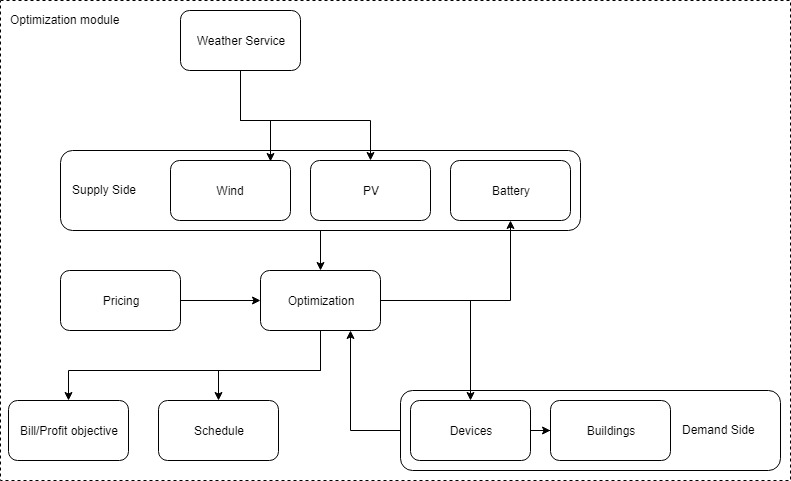
\includegraphics[width=0.7\columnwidth]{Optimization.jpg}
	\caption{The Optimization module}
	\label{img:optimization_module}
\end{figure}

Unlike other modules, optimization is not a class, but only an API by optimizaion\_app. By entering optimize under url \texttt{0.0.0.0:4070}, a dictionary of data is output on User Interface, containing for each building a CED schedule and bill, and profit for stakeholder. It also update battery status and energy level, and update CED start and end time inside demand API.

The current optimization model is designed for only 2 houses only, but unlimited number of devices can be added. The generation price for Wind and PV modules, and maximum grid power exchange are currently hard coded, which are 2 and 1 cents per kWh and -200/200 kWh. Due to 1-hour dynamic pricing, time step is 1 and  time scale is 24 hours.

With the help of Gurobi\cite{Gurobi}, this mathematical model can be solved once element constraints are well defined; the first and most important is balance between demand and supply, blackout will otherwise result with 5\% imbalance:\newline

\[\displaystyle \sum_{p}^{\\plants} gen[t] - \sum_{d}^{\\devices} demand[t] + battery[t-1] + grid[t] == 0\]  

Devices, which are UC and CED are also input variables and constraints are mentioned in demand side part; to battery, these must be considered:
\newline
 \[charge[t] == 1, \; if \;0 < gen[t] - demand[t] < E_{CH}^{SPEC}\]
 \newline
 \[discharge[t] == 1, \; if \;E_{DCH}^{SPEC} < gen[t] - demand[t] < 0 \]
 \newline
\[idle[t] == 1, \; if \;gen[t] - demand[t] > E_{CH}^{SPEC} \;or\; gen[t] - demand[t] < E_{DCH}^{SPEC} \]
\newline
\[Energy_charge[t] = charge[t] * (gen[t] - demand[t]) \]
\newline
\[Energy_discharge[t] = discharge[t] * (gen[t] - demand[t]) \]
\newline
\begin{align*}
Energy\_level[t+1] = Energy\_level[t] + \delta \times \eta \times Energy\_charge[t] \\
+ \frac{\delta \times \ Energy\_discharge[t]}{\eta} -\delta \times Energy\_selfdischarge
\end{align*}
\newline
\[\displaystyle \sum_{t}^{\\time} Energy\_charge[t] + Energy_discharge[t] == 0\] 
\newline
\[Energy\_level[t=0] == Energy\_level[t=24] \]
	
However, battery constraints are failed to cooperate with other constraints inside gurobi model. Another attempt was building a separate model for battery after optimize the whole system without battery; the objective function is hence maximize the amount of energy exchanged within battery, by doing so, battery is used the most during day, this strategy fails in logic of profit optimization by storing energy at high price and use at low price sometimes. 
\[\displaystyle \sum_{t}^{\\time} Energy\_level[t] == 0\]
and
\[\displaystyle \max\sum_{t}^{\\time} |Energy\_level[t]|\]

Finally, logic based calculation is used to assign battery status and battery energy level after the sample optimized model, the profit (cents) is hence re-calculated, including 10\% tax as: 

\[\displaystyle 0.9 \times \sum_{t}^{\\time} gen[t]*tariff[t] - Wind\_revenue - PV\_revenue\]

in which, 

$\displaystyle Wind\_revenue = \sum_{t}^{\\time} Wind\_out[t] \times Wind\_price$

$\displaystyle PV\_revenue = \sum_{t}^{\\time} PV\_out[t] \times PV\_price$

and bill (cents) is calculated as:
$\displaystyle \sum_{t}^{\\time} demand[t] \times tariff[t]$
\begin{figure}[H]
	\centering
	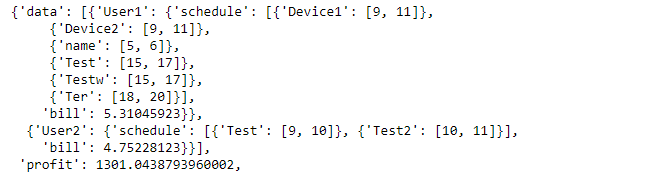
\includegraphics[width=0.9\columnwidth]{optimization2.PNG}
	\caption{Schedule, profit and bill}
	\label{img:profit_bill}
\end{figure}

It is clearly that, the profit of stakeholder is re-calculated as 1300cents/day instead of objective value model.objval, because it is assumed that all the generated energy is sold at tariff[t], either to grid or to houses. One more reason for these small values are the dynamic tariff from entsoe, they are indeed roughly 2-4 cent/kWh, which is too small, therefore, the profit is somehow negative due to higher producing price of renewable energy. 

To one user, there is a list containing name of CED with start and end time, which is afterwards fed to device and display units. Battery energy level and status are also output as: 

\begin{figure}[H]
	\centering
	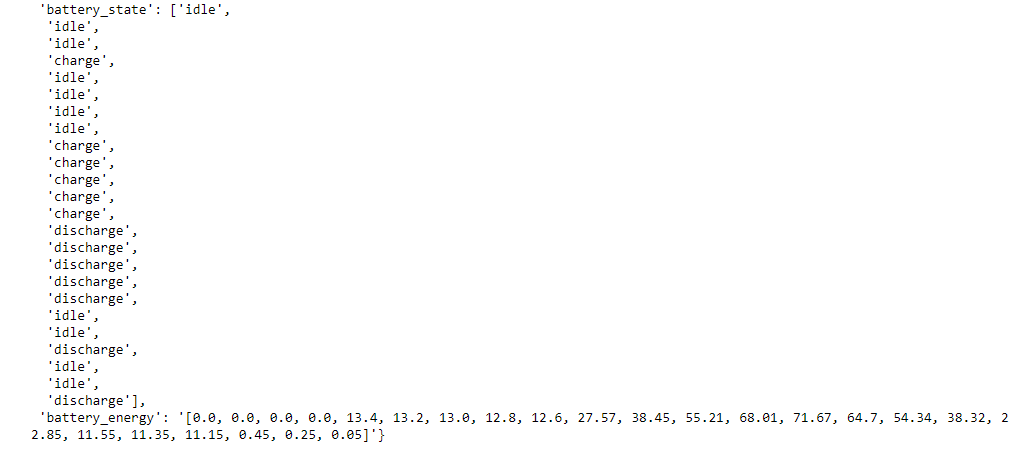
\includegraphics[width=1\columnwidth]{optimization.PNG}
	\caption{Energy level and status of battery}
	\label{img: optimized_bat}
\end{figure}
The result of optimization service is then shown on Web Interface for better observation; other attempt to perform as chart for higher visualization quality is unavailable due to shortage of time.
\begin{figure}[H]
	\centering
	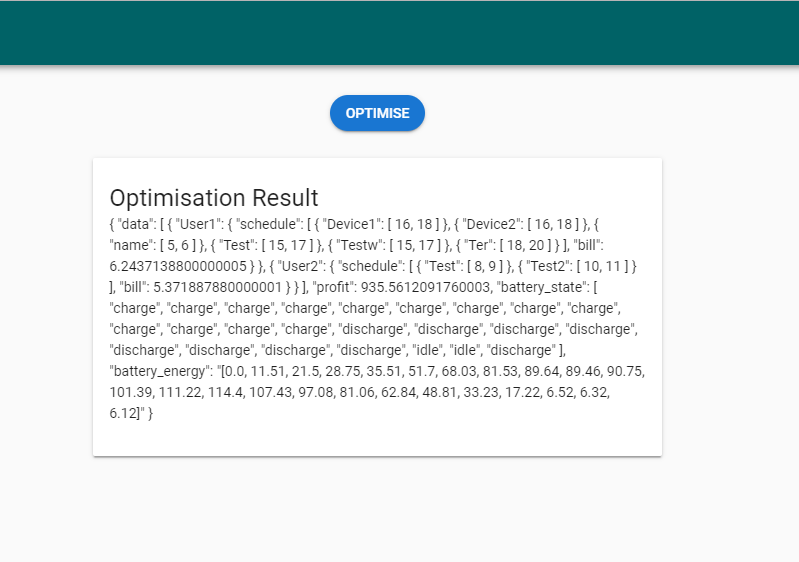
\includegraphics[width=1\columnwidth]{optimization3.PNG}
	\caption{Optimization output on UI}
	\label{img: optimized_UI}
\end{figure}

Theoretically, battery should perform supportive role in the microgrid while storing and powering excess energy of renewable modules. The beginning level of battery should be 0, and during day, charge and discharge repeatedly appear. Current level and status are also updated to supply\_side and UI. In case of wrong input, leading to unsolvable model, optimization will output None only. 

\section{Visualization}
We have designed our front end to be as user friendly as possible. When user accesses our website, they are directed to our welcome page. We have setup a simple navigation system where user can jump to any page by clicking respective tabs in the left hand pane.

Energy generation, pricing and demand profiles are available as different tabs to provide a modular representation. In components management tab user can add and view different types of generators and consumer units in very simple manner as described later.
\begin{figure}[H]
\centering
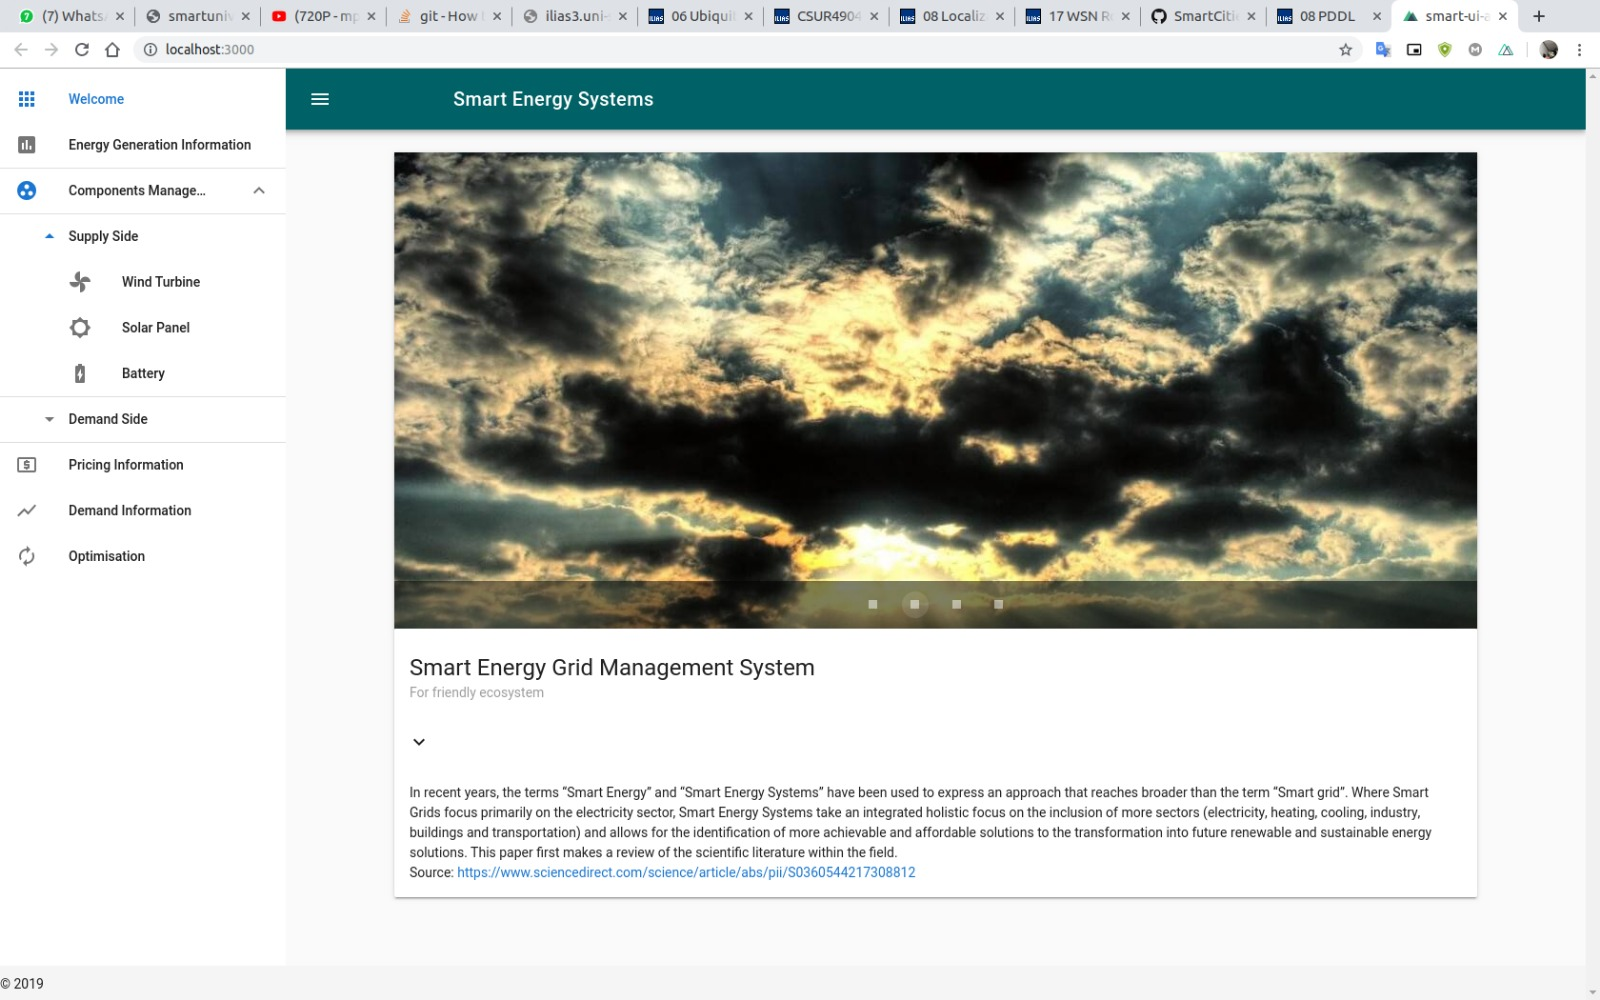
\includegraphics[width=0.8\textwidth]{actual/visualization/introduction.jpeg}
\caption{Welcome page} 
\label{figv1}
\end{figure}
First we talk about the energy generation information tab. It shows three graphs. The leftmost one shows total energy generation in KW for current day. The middle graph shows forecast of energy generation for next 24 hours. Graph on the right shows history of energy generation for current day with best suited resolution. For consistency and ease of comprehension Wind energy is always shown in blue and solar energy in yellow.
\begin{figure}[H]
\centering
\includegraphics[width=0.8\textwidth]{{"actual/visualization/energy generation information"}.jpeg}
\caption{Energy generation information tab} 
\label{figv2}
\end{figure}
Next we have component management section. It consists of multiple tabs and two subsections, namely Supply and Demand. Supply subsection consists of three tabs; Wind turbine, solar panel and battery. In Demand subsection has building and device tabs. By default when user navigates to a tab she can see all available units in listed format. All of this tabs lets user intuitively add new units. This is achieved by clicking on add button of corresponding unit. Only exception is battery tab.
First we start with the supply section. For Wind turbine view all as list and add a new Wind turbine is presented below.
\begin{figure}[H]
\centering
\includegraphics[width=0.8\textwidth]{{"actual//visualization//wind turbine"}.jpeg}
\caption{Wind turbine tab} 
\label{figv3}
\end{figure}
We assume Wind turbine is active by default. Location selection from a predefined list of options and Ra parameter are the only thing asked.  
\begin{figure}[H]
\centering
\includegraphics[width=0.8\textwidth]{{"actual/visualization/add wind turbine"}.jpeg}
\caption{Add Wind turbine popup} 
\label{figv4}
\end{figure}
We do the same thing for solar panels too.
\begin{figure}[H]
\centering
\includegraphics[width=0.8\textwidth]{{"actual/visualization/solar panel"}.jpeg}
\caption{Solar panel tab} 
\label{figv5}
\end{figure}
We assume solar panel is also active by default. Along with location; area, maximum energy generation capacity and angle of module is asked from user. All inputs are mandatory.  
\begin{figure}[H]
\centering
\includegraphics[width=0.8\textwidth]{{"actual/visualization/add solar panel"}.jpeg}
\caption{Add solar panel popup} 
\label{figv6}
\end{figure}
Battery unit shows current state,power level,maximum charge capacity,maximum discharge capacity,maximum energy capacity etc. 
\begin{figure}[H]
\centering
\includegraphics[width=0.8\textwidth]{{"actual/visualization/Batterystaus"}.jpeg}
\caption{Battery Status tab} 
\label{figv5}
\end{figure}
We can update the battery status from the Update battery pop up.
\begin{figure}[H]
\centering
\includegraphics[width=0.8\textwidth]{{"actual/visualization/Updatebattery"}.jpeg}
\caption{Update Battery status popup} 
\label{figv5}
\end{figure}
For Demand section we have the same functionality to ensure a proper blend of functionality and consistency with user experience.

\begin{figure}[H]
\centering
\includegraphics[width=0.8\textwidth]{{"actual/visualization/buildings"}.jpeg}
\caption{Building tab} 
\label{figv7}
\end{figure}

We only ask for name from user here so that user can add device(s) to corresponding building in device tab in meaningful manner.
\begin{figure}[H]
\centering
\includegraphics[width=0.8\textwidth]{{"actual/visualization/add building"}.jpeg}
\caption{Add building popup} 
\label{figv8}
\end{figure}

For devices we have a small change in representation. In this tab user must select a building for which devices are to be listed. Initially we select a default building for which devices are shown.

\begin{figure}[H]
\centering
\includegraphics[width=0.78\textwidth]{{"actual/visualization/device"}.jpeg}
\caption{Device tab} 
\label{figv9}
\end{figure}

When user clicks on add device button it is assumed user is trying to add a device to a building for which other devices are being displayed. Asked parameters here are name, EST, LET, and LOT in 24 hour format, power(kW), initial start and stop time.
\begin{figure}[H]
\centering
\includegraphics[width=0.7\textwidth]{{"actual/visualization/add device"}.jpeg}
\caption{Add device popup} 
\label{figv10}
\end{figure}


After this we come to pricing information tab. This tab gives information on pricing on hourly resolution for current day, next 24 hours and tomorrow. The relevant information is selected from a list of options menu. All currency information is in Euro.

\begin{figure}[H]
\centering
\includegraphics[width=0.7\textwidth]{{"actual/visualization/todays pricing trend"}.jpeg}
\caption{Pricing trend for current day } 
\label{figv11}
\end{figure}

\begin{figure}[H]
\centering
\includegraphics[width=0.7\textwidth]{{"actual/visualization/price trend for next 24 - forecast"}.jpeg}
\caption{Pricing trend for next 24 hour} 
\label{figv12}
\end{figure}

\begin{figure}[H]
\centering
\includegraphics[width=0.7\textwidth]{{"actual/visualization/pricing trend tomorrow - forecast"}.jpeg}
\caption{Pricing trend for next day} 
\label{figv13}
\end{figure}

Demand information tab shows consumption information for buildings as whole or their respective devices. Name of buildings and devices can be selected from drop down menu. All the information is in kW in hourly resolution.

\begin{figure}[H]
\centering
\includegraphics[width=0.7\textwidth]{{"actual/visualization/demand"}.jpeg}
\caption{Demand for each building} 
\label{figv14}
\end{figure}

\begin{figure}[H]
\centering
\includegraphics[width=0.7\textwidth]{{"actual/visualization/demand per device"}.jpeg}
\caption{Demand for each device} 
\label{figv15}
\end{figure}

\section{Outlook}
\begin{itemize}
	\item Change user's location: this project currently assumes user is at university of Stuttgart, so that all the information processed within are from location Stuttgart, Germany. Later on, user can freely choose city and country for personal use. However, we also have to limit and update the number of European countries in order to fit with the entsoe-py database; presently, entsoe contains 33 bidding zones and 42 countries'/regions names and this number will changed regularly  overtime.\cite{Entsoe}

	\item There should be dynamic in scaling, unlimited number of buildings/inhabitants instead of 2 currently, for instance, and all hard coded values, such as producing price of Wind and PV etc could be set by user, or an independent decision making unit.
	
	\item There should be more options to optimize the micro-grid, the future target is to use battery as an utility to buy electricity at low price and sell it at high price, not just to store excess electricity for grid-only use.
	
	\item There should be a logic check mechanism for correct-only input values, the optimization service is hence always accessible.
	
	\item There should be separate interface for users as inhabitants and as stakeholders, since they play different roles in the system with different targets, profits and contributions.
	
	\item There should be an app for the ease of nowaday usage.
\end{itemize}

\section{Conclusion}
Without any major problems, this project runs well in presentation and for longer usage. It covers all the tasks assigned during the course, featuring an analyzing tool for smart micro-grid. As a reason of
simple and small model, this project still has scaling limitation.

%
% ---- Bibliography ----
%
\begin{thebibliography}{9}
\bibitem{Efficiency} 
Di Zhang, Nilay Shah, L.G.P.:
\textit{ Efficient energy consumption and operation management in a smart building with microgrid. Energy Conversion and Management 74, (2013)}. 

\bibitem{Microgrid} 
A. A. Salam, A.M., Hannan, M.A.: 
\textit{ echnical challenges on microgrids. ARPN Journalof Engineering and Applied Sciences3, 64–69 (2008)}. 

\bibitem{Bottlepy} 
Bottlepy,
\texttt{https://bottlepy.org/docs/dev/tutorial.html}. 
[Online; accessed 20.07.2019].

\bibitem{Irradiance} 
PVeducation.org, Solar Radiation on a Tilted Angle,
\texttt{https://www.pveducation.org/pvcdrom/properties-of-sunlight/solar-radiation-on-a-tilted-surface}. 
[Online; accessed 20.07.2019].

\bibitem{Entsoe} 
Entsoe, 
\texttt{ https://github.com/EnergieID/entsoe-py/blob/master/entsoe/mappings.py}. 
[Online; accessed 20.07.2019].

\bibitem{Opsd} 
Opsd, 
\texttt{ https://data.open-power-system-data.org/householddata/2017−11−10}. 
[Online; accessed 20.07.2019].
 
\bibitem{Weatherbit.io} 
Weatherbit.io, 
\texttt{ https://www.weatherbit.io/about}. 
[Online; accessed 20.07.2019]. 

\bibitem{Vuejs} 
Vuejs, 
\texttt{ https://vuetifyjs.com/en/}. 
[Online; accessed 20.07.2019]. 

\bibitem{Gurobi} 
Gurobi solver, 
\texttt{ https://www.gurobi.com/downloads/end-user-license-agreement-academic/}. 
[Online; accessed 20.07.2019]. 

\bibitem{Ilche} 
IlcheGeorgievski, M.A.: SmartEnergySystems: introduction to supply side and demand side
\texttt{https://ilias3.uni-stuttgart.de/gotoUniStuttgartfile1670605download.html,} 
[Online; accessed 20.07.2019].

\end{thebibliography}
 
\end{document}

All links were last followed on July 20, 2019.

\end{document}